\documentclass{article}
\usepackage{amsmath, amsthm, amsfonts}
\usepackage{centernot}
\usepackage{caption}
\usepackage{tikz}
\usetikzlibrary{automata, positioning, arrows}
\tikzset{
->, % makes the edges directed
>=stealth', % makes the arrow heads bold
node distance=3cm, % specifies the minimum distance between two nodes. Change if necessary.
every state/.style={thick, fill=gray!10}, % sets the properties for each ’state’ node
initial text=$ $, % sets the text that appears on the start arrow
}
\usepackage{float}
\author{Mostafa Hassanein}
\title{
  MTH-682 Automata \\
  Assignment (1): Regular Languages}
\date{22 October 2025}
\begin{document}
\maketitle
\newpage

\section*{1.4}

Each of the following languages is the intersection of two simpler languages. In
each part, construct DFAs for the simpler languages, then combine them using the
construction discussed in footnote 3 (page 46) to give the state diagram of a DFA
for the language given. In all parts, $\Sigma= \{ a, b \}$.

\subsection*{c. $L = \{ w| w \text{ has an even number of } a \text{'s and one or two } b \text{'s} \}$}

\begin{center}
  \underline{Solution:}
\end{center}

\underline{Languages:}
\newline

$L = L_1 \cap L_2$

$L_1 = \{ w| \:w \text{ has an even number of} \: a \text{'s} \}$

$L_2 = \{ w| \:w \text{ has one or two} \: b \text{'s} \}$
\newline

\underline{Automata:}

\begin{figure}[H]
  \centering
  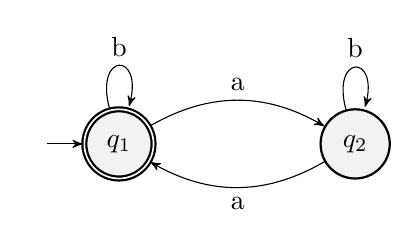
\begin{tikzpicture}
    \node[state, initial, accepting] (q1) {$q_1$};
    \node[state, right of=q1] (q2) {$q_2$};
    \draw 
    (q1) edge[bend left, above] node{a} (q2)
    (q1) edge[loop above] node{b} (q1)
    (q2) edge[bend left, below] node{a} (q1)
    (q2) edge[loop above] node{b} (q2);
  \end{tikzpicture}
  \caption{$DFA_{L_1}$}
\end{figure}

\begin{figure}[H]
  \centering % centers the figure
  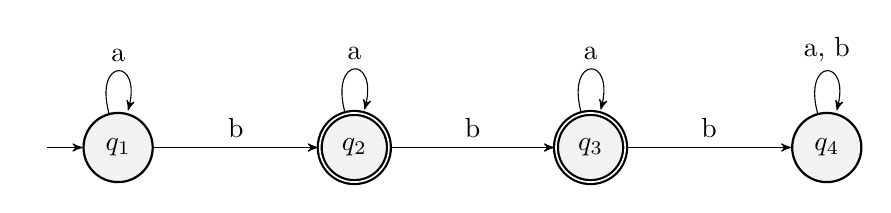
\begin{tikzpicture}
    \node[state, initial] (q1) {$q_1$};
    \node[state, accepting, right of=q1] (q2) {$q_2$};
    \node[state, accepting, right of=q2] (q3) {$q_3$};
    \node[state, right of=q3] (q4) {$q_4$};
    \draw 
    (q1) edge[loop above] node{a} (q1)
    (q1) edge[above] node{b} (q2)
    (q2) edge[loop above] node{a} (q2)
    (q2) edge[above] node{b} (q3)
    (q3) edge[loop above] node{a} (q3)
    (q3) edge[above] node{b} (q4)
    (q4) edge[loop above] node{a, b} (q4);
  \end{tikzpicture}
  \caption{$DFA_{L_2}$}
\end{figure}

\begin{table}[H]
\centering
\begin{tabular}{|c|c|c|}
\hline
\textbf{State} & \textbf{a} & \textbf{b} \\
\hline
$q_{11}$ & $q_{21}$ & $q_{12}$ \\
$q_{21}$ & $q_{11}$ & $q_{22}$ \\
$q_{12}$ & $q_{22}$ & $q_{13}$ \\
$q_{22}$ & $q_{12}$ & $q_{23}$ \\
$q_{23}$ & $q_{13}$ & $q_{24}$ \\
$q_{13}$ & $q_{23}$ & $q_{14}$ \\
$q_{24}$ & $q_{14}$ & $q_{24}$ \\
$q_{14}$ & $q_{24}$ & $q_{14}$ \\
\hline
\end{tabular}
\caption{Transition Table}
\end{table}

\begin{figure}[H]
  \centering % centers the figure
  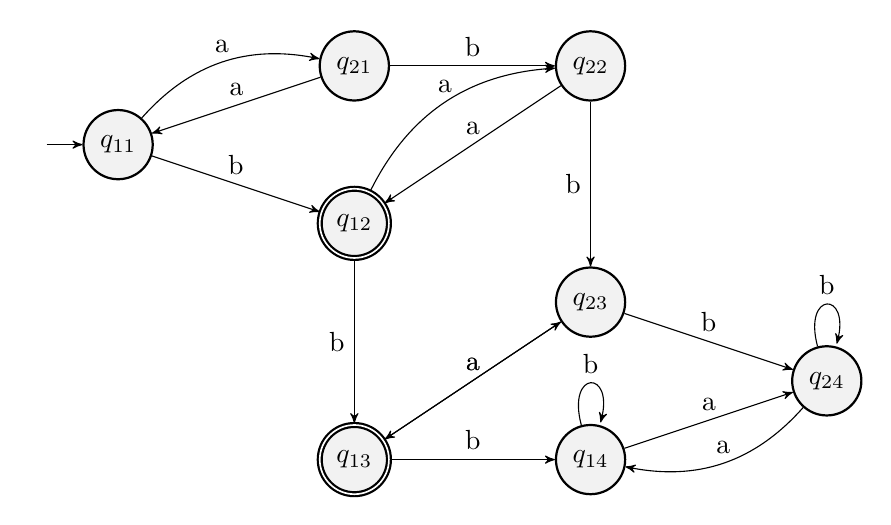
\begin{tikzpicture}
    \node[state, initial] (q11) {$q_{11}$};
    \node[state, right of=q11, yshift=1cm] (q21) {$q_{21}$};
    \node[state, accepting, right of=q11, yshift=-1cm] (q12) {$q_{12}$};
    \node[state, right of=q21] (q22) {$q_{22}$};
    \node[state, below of=q22] (q23) {$q_{23}$};
    \node[state, accepting, below of=q12] (q13) {$q_{13}$};
    \node[state, right of=q23, yshift=-1cm] (q24) {$q_{24}$};
    \node[state, right of=q13] (q14) {$q_{14}$};
    \draw 
    (q11) edge[bend left, above] node{a} (q21)
    (q11) edge[above] node{b} (q12)
    (q21) edge[above] node{a} (q11)
    (q21) edge[above] node{b} (q22)
    (q22) edge[above] node{a} (q12)
    (q22) edge[left] node{b} (q23)
    (q23) edge[above] node{a} (q13)
    (q23) edge[above] node{b} (q24)
    (q13) edge[above] node{a} (q23)
    (q13) edge[above] node{b} (q14)
    (q24) edge[bend left, above] node{a} (q14)
    (q24) edge[loop above] node{b} (q24)
    (q14) edge[above] node{a} (q24)
    (q14) edge[loop above] node{b} (q14)
    (q12) edge[bend left, above] node{a} (q22)
    (q12) edge[left] node{b} (q13);
  \end{tikzpicture}
  \caption{$DFA_{L}$}
\end{figure}


\subsection*{f. $L = \{ w| w \text{ has an odd number of } a \text{'s and ends with a } b \}$}

\begin{center}
  \underline{Solution:}
\end{center}

\underline{Languages:}
\newline

$L = L_1 \cap L_2$

$L_1 = \{ w| \:w \text{ has an odd number of} \: a \text{'s} \}$

$L_2 = \{ w| \:w \text{ ends with a} \: b \}$
\newline

\underline{Automata:}

\begin{figure}[H]
  \centering % centers the figure
  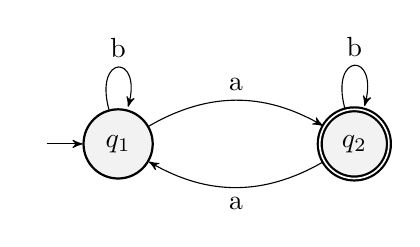
\begin{tikzpicture}
    \node[state, initial] (q1) {$q_1$};
    \node[state, accepting, right of=q1] (q2) {$q_2$};
    \draw 
    (q1) edge[bend left, above] node{a} (q2)
    (q1) edge[loop above] node{b} (q1)
    (q2) edge[bend left, below] node{a} (q1)
    (q2) edge[loop above] node{b} (q2);
  \end{tikzpicture}
  \caption{$DFA_{L_1}$}
\end{figure}

\begin{figure}[H]
  \centering % centers the figure
  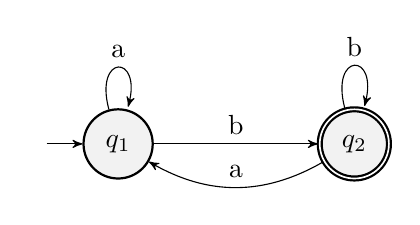
\begin{tikzpicture}
    \node[state, initial] (q1) {$q_1$};
    \node[state, accepting, right of=q1] (q2) {$q_2$};
    \draw 
    (q1) edge[loop above] node{a} (q1)
    (q1) edge[above] node{b} (q2)
    (q2) edge[bend left,above] node{a} (q1)
    (q2) edge[loop above] node{b} (q2);
  \end{tikzpicture}
  \caption{$DFA_{L_2}$}
\end{figure}

\begin{table}[H]
\centering
\begin{tabular}{|c|c|c|}
\hline
\textbf{State} & \textbf{a} & \textbf{b} \\
\hline
$q_{11}$ & $q_{21}$ & $q_{12}$ \\
$q_{12}$ & $q_{21}$ & $q_{12}$ \\
$q_{21}$ & $q_{11}$ & $q_{22}$ \\
$q_{22}$ & $q_{11}$ & $q_{22}$ \\
\hline
\end{tabular}
\caption{Transition Table}
\end{table}

\begin{figure}[H]
  \centering % centers the figure
  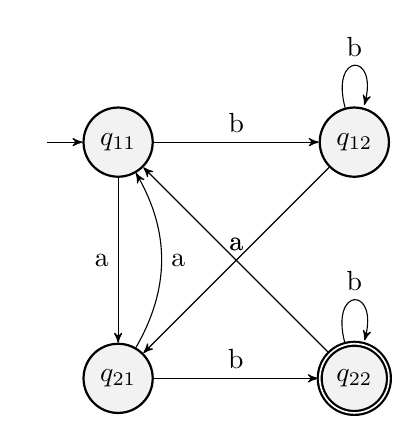
\begin{tikzpicture}
    \node[state, initial] (q11) {$q_{11}$};
    \node[state, right of=q11] (q12) {$q_{12}$};
    \node[state, below of=q11] (q21) {$q_{21}$};
    \node[state, accepting, right of=q21] (q22) {$q_{22}$};
    \draw 
    (q11) edge[left] node{a} (q21)
    (q11) edge[above] node{b} (q12)
    (q12) edge[above] node{a} (q21)
    (q12) edge[loop above] node{b} (q12)
    (q21) edge[bend right, right] node{a} (q11)
    (q21) edge[above] node{b} (q22)
    (q22) edge[above] node{a} (q11)
    (q22) edge[loop above] node{b} (q22);
  \end{tikzpicture}
  \caption{$DFA_{L}$}
\end{figure}


\section*{1.5}
Each of the following languages is the complement of a simpler language. In each
part, construct a DFA for the simpler language, then use it to give the state diagram
of a DFA for the language given. In all parts, $\Sigma = \{a, b\}$.

\subsection*{c. $L = \{ w| w \text{ contains neither the substrings } ab \text{ nor } ba\}$}

\begin{center}
  \underline{Solution:}
\end{center}

$L^c = \{ w| w \text{ contains the substring } ab \text{ or } ba \}$
\newline

\begin{figure}[H]
  \centering
  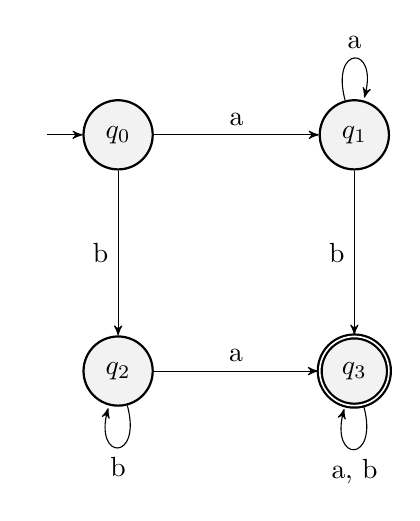
\begin{tikzpicture}
    \node[state, initial] (q0) {$q_0$};
    \node[state, right of=q0] (q1) {$q_1$};
    \node[state, below of=q0] (q2) {$q_2$};
    \node[state, accepting, right of=q2] (q3) {$q_3$};
    \draw 
    (q0) edge[above] node{a} (q1)
    (q0) edge[left] node{b} (q2)
    (q1) edge[loop above] node{a} (q1)
    (q1) edge[left] node{b} (q3)
    (q2) edge[loop below] node{b} (q2)
    (q2) edge[above] node{a} (q3)
    (q3) edge[loop below] node{a, b} (q3);
  \end{tikzpicture}
  \caption{$DFA_{L^c}$}
\end{figure}

\begin{figure}[H]
  \centering
  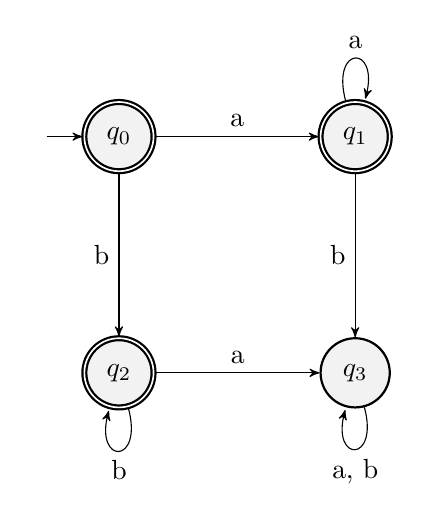
\begin{tikzpicture}
    \node[state, initial, accepting] (q0) {$q_0$};
    \node[state, accepting, right of=q0] (q1) {$q_1$};
    \node[state, accepting, below of=q0] (q2) {$q_2$};
    \node[state, right of=q2] (q3) {$q_3$};
    \draw 
    (q0) edge[above] node{a} (q1)
    (q0) edge[left] node{b} (q2)
    (q1) edge[loop above] node{a} (q1)
    (q1) edge[left] node{b} (q3)
    (q2) edge[loop below] node{b} (q2)
    (q2) edge[above] node{a} (q3)
    (q3) edge[loop below] node{a, b} (q3);
  \end{tikzpicture}
  \caption{$DFA_{L}$}
\end{figure}


\subsection*{f. $L = \{ w| w \text{ is any string not in } a^* \cup b^* \}$}

\begin{center}
  \underline{Solution:}
\end{center}

$L^c = a^* \cup b^* = \{ w| w \text{ contains only } a \text{'s or only } b \text{'s (including } \varepsilon \text{)} \}$
\newline

\begin{figure}[H]
  \centering
  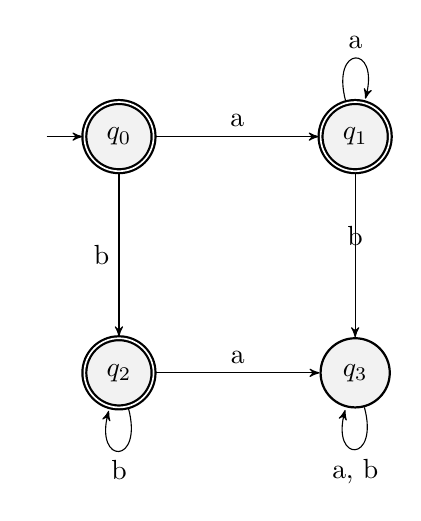
\begin{tikzpicture}
    \node[state, initial, accepting] (q0) {$q_0$};
    \node[state, accepting, right of=q0] (q1) {$q_1$};
    \node[state, accepting, below of=q0] (q2) {$q_2$};
    \node[state, right of=q2] (q3) {$q_3$};
    \draw 
    (q0) edge[above] node{a} (q1)
    (q0) edge[left] node{b} (q2)
    (q1) edge[loop above] node{a} (q1)
    (q1) edge[above] node{b} (q3)
    (q2) edge[loop below] node{b} (q2)
    (q2) edge[above] node{a} (q3)
    (q3) edge[loop below] node{a, b} (q3);
  \end{tikzpicture}
  \caption{$DFA_{L^c}$}
\end{figure}

\begin{figure}[H]
  \centering
  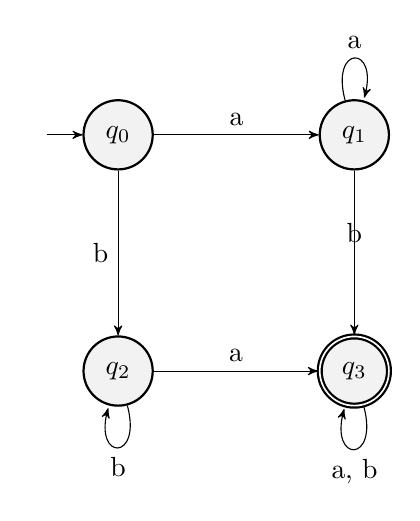
\begin{tikzpicture}
    \node[state, initial] (q0) {$q_0$};
    \node[state, right of=q0] (q1) {$q_1$};
    \node[state, below of=q0] (q2) {$q_2$};
    \node[state, accepting, right of=q2] (q3) {$q_3$};
    \draw 
    (q0) edge[above] node{a} (q1)
    (q0) edge[left] node{b} (q2)
    (q1) edge[loop above] node{a} (q1)
    (q1) edge[above] node{b} (q3)
    (q2) edge[loop below] node{b} (q2)
    (q2) edge[above] node{a} (q3)
    (q3) edge[loop below] node{a, b} (q3);
  \end{tikzpicture}
  \caption{$DFA_{L}$}
\end{figure}


\section*{1.6}
Give state diagrams of DFAs recognizing the following languages. In all parts, the
alphabet is ${0,1}$.

\subsection*{a. $L = \{ w| w \text{ begins with a } 1 \text{ and ends with a } 0 \}$}

\begin{center}
  \underline{Solution:}
\end{center}

\begin{figure}[H]
  \centering
  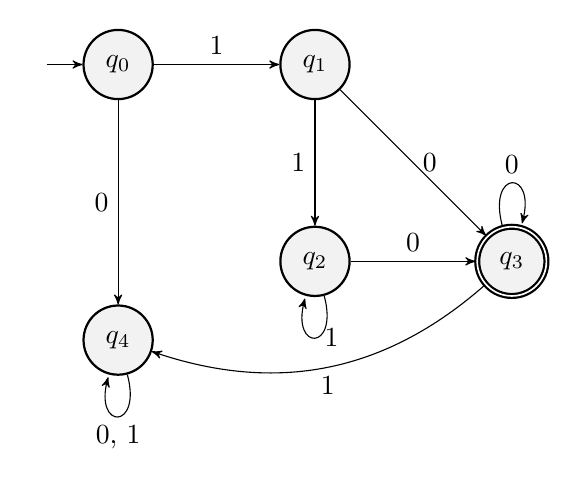
\begin{tikzpicture}[node distance=2.5cm]
    \node[state, initial] (q0) {$q_0$};
    \node[state, right of=q0] (q1) {$q_1$};
    \node[state, below of=q1] (q2) {$q_2$};
    \node[state, accepting, right of=q2] (q3) {$q_3$};
    \node[state, below of=q0, yshift=-1cm] (q4) {$q_4$};
    \draw 
    (q0) edge[above] node{1} (q1)
    (q0) edge[left] node{0} (q4)
    (q1) edge[right] node{0} (q3)
    (q1) edge[left] node{1} (q2)
    (q2) edge[above] node{0} (q3)
    (q2) edge[loop below, right] node{1} (q2)
    (q3) edge[loop above] node{0} (q3)
    (q3) edge[bend left, below] node{1} (q4)
    (q4) edge[loop below] node{0, 1} (q4);
  \end{tikzpicture}
  \caption{$DFA_{L}$}
\end{figure}

\subsection*{b. $L = \{ w| w \text{ contains at least three } 1 \text{'s} \}$}

\begin{center}
  \underline{Solution:}
\end{center}

\begin{figure}[H]
  \centering
  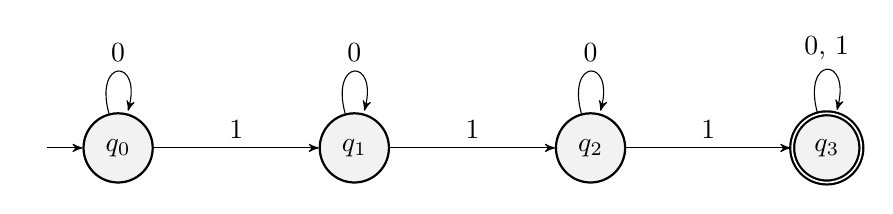
\begin{tikzpicture}[node distance=3cm]
    \node[state, initial] (q0) {$q_0$};
    \node[state, right of=q0] (q1) {$q_1$};
    \node[state, right of=q1] (q2) {$q_2$};
    \node[state, accepting, right of=q2] (q3) {$q_3$};
    \draw 
    (q0) edge[loop above] node{0} (q0)
    (q0) edge[above] node{1} (q1)
    (q1) edge[loop above] node{0} (q1)
    (q1) edge[above] node{1} (q2)
    (q2) edge[loop above] node{0} (q2)
    (q2) edge[above] node{1} (q3)
    (q3) edge[loop above] node{0, 1} (q3);
  \end{tikzpicture}
  \caption{$DFA_{L}$}
\end{figure}

\subsection*{c. $L = \{  w| w \text{ contains the substring } 0101 \text{ (i.e., w = x0101y for some x and y)} \}$}

\begin{center}
  \underline{Solution:}
\end{center}

\begin{figure}[H]
  \centering
  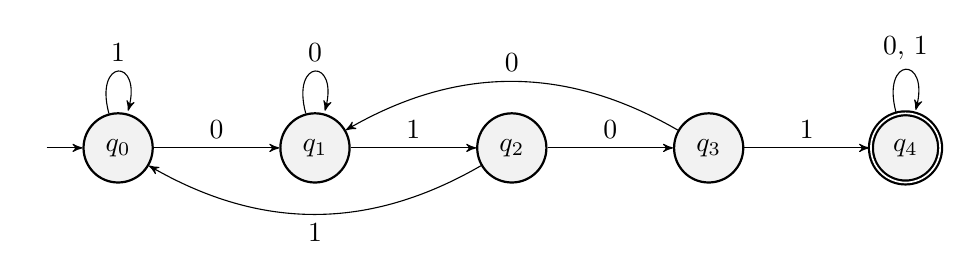
\begin{tikzpicture}[node distance=2.5cm]
    \node[state, initial] (q0) {$q_0$};
    \node[state, right of=q0] (q1) {$q_1$};
    \node[state, right of=q1] (q2) {$q_2$};
    \node[state, right of=q2] (q3) {$q_3$};
    \node[state, accepting, right of=q3] (q4) {$q_4$};
    \draw 
    (q0) edge[loop above] node{1} (q0)
    (q0) edge[above] node{0} (q1)
    (q1) edge[loop above] node{0} (q1)
    (q1) edge[above] node{1} (q2)
    (q2) edge[bend left, below] node{1} (q0)
    (q2) edge[above] node{0} (q3)
    (q3) edge[bend right, above] node{0} (q1)
    (q3) edge[above] node{1} (q4)
    (q4) edge[loop above] node{0, 1} (q4);
  \end{tikzpicture}
  \caption{$DFA_{L}$}
\end{figure}


\section*{1.7}
Give state diagrams of NFAs with the specified number of states recognizing each
of the following languages. In all parts, the alphabet is $\{0,1\}$.

\subsection*{b. $L = \{  w| w \text{ contains the substring } 0101 \text{ (i.e., w = x0101y for some x and y)} \}$. 
\newline \indent 
$States = 5$.}

\begin{center}
  \underline{Solution:}
\end{center}

\begin{figure}[H]
  \centering
  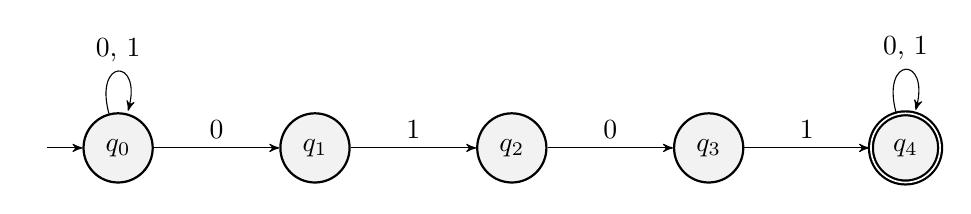
\begin{tikzpicture}[node distance=2.5cm]
    \node[state, initial] (q0) {$q_0$};
    \node[state, right of=q0] (q1) {$q_1$};
    \node[state, right of=q1] (q2) {$q_2$};
    \node[state, right of=q2] (q3) {$q_3$};
    \node[state, accepting, right of=q3] (q4) {$q_4$};
    \draw 
    (q0) edge[loop above] node{0, 1} (q0)
    (q0) edge[above] node{0} (q1)
    (q1) edge[above] node{1} (q2)
    (q2) edge[above] node{0} (q3)
    (q3) edge[above] node{1} (q4)
    (q4) edge[loop above] node{0, 1} (q4);
  \end{tikzpicture}
  \caption{$NFA_{L}$}
\end{figure}

\subsection*{e. $L$ is the language of the regular expression $0^*1^*0^+$.
\newline \indent 
$States = 3$.}

\begin{center}
  \underline{Solution:}
\end{center}

\begin{figure}[H]
  \centering
  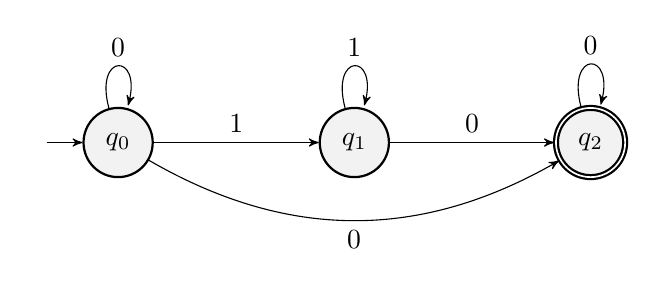
\begin{tikzpicture}[node distance=3cm]
    \node[state, initial] (q0) {$q_0$};
    \node[state, right of=q0] (q1) {$q_1$};
    \node[state, accepting, right of=q1] (q2) {$q_2$};
    \draw 
    (q0) edge[loop above] node{0} (q0)
    (q0) edge[bend right, below] node{0} (q2)
    (q0) edge[above] node{1} (q1)
    (q1) edge[loop above] node{1} (q1)
    (q1) edge[above] node{0} (q2)
    (q2) edge[loop above] node{0} (q2);
  \end{tikzpicture}
  \caption{$NFA_{L}$}
\end{figure}


\section*{1.8}
Use the construction in the proof of Theorem $1.45$ to give the state diagrams of
NFAs recognizing the union of the languages described in:
\subsection*{a. Exercises 1.6.a and 1.6.b}

\begin{center}
  \underline{Solution:}
\end{center}

\begin{figure}[H]
  \centering
  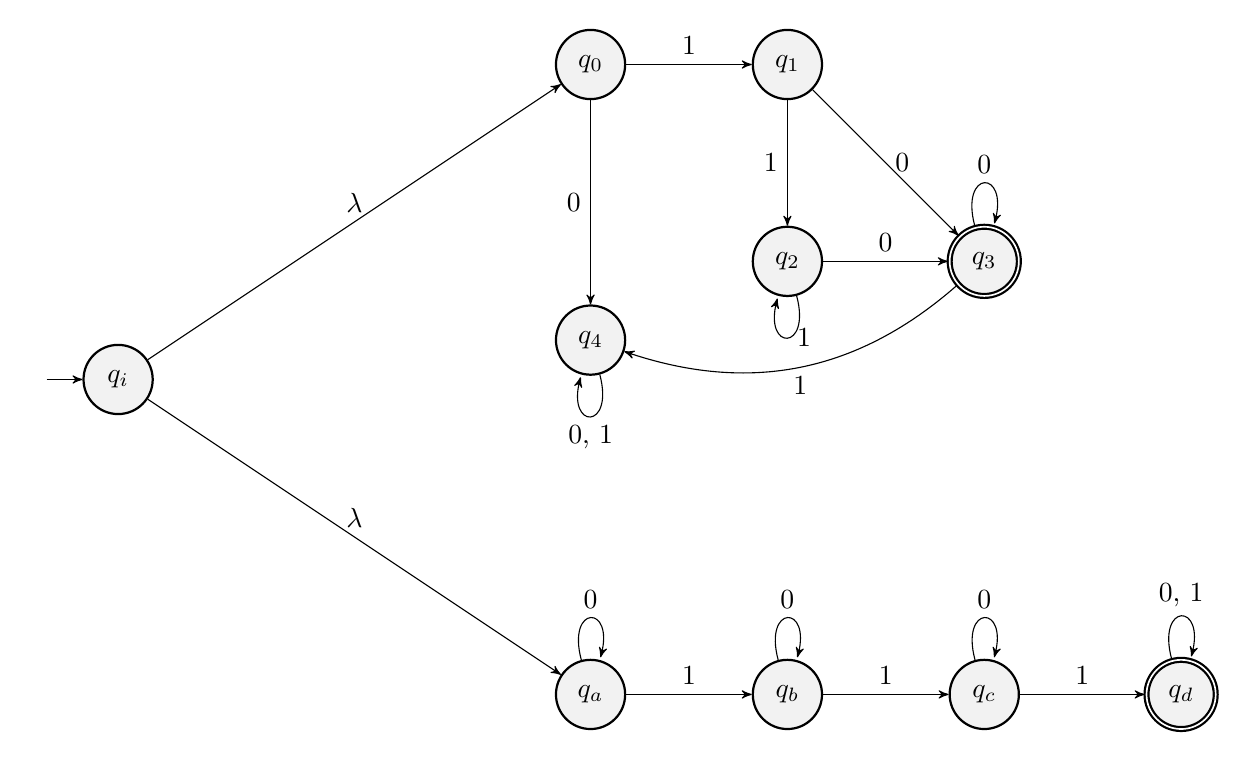
\begin{tikzpicture}[node distance=2.5cm]
    % DFA 1
    \node[state] (q0) {$q_0$};
    \node[state, right of=q0] (q1) {$q_1$};
    \node[state, below of=q1] (q2) {$q_2$};
    \node[state, accepting, right of=q2] (q3) {$q_3$};
    \node[state, below of=q0, yshift=-1cm] (q4) {$q_4$};
    \draw 
    (q0) edge[above] node{1} (q1)
    (q0) edge[left] node{0} (q4)
    (q1) edge[right] node{0} (q3)
    (q1) edge[left] node{1} (q2)
    (q2) edge[above] node{0} (q3)
    (q2) edge[loop below, right] node{1} (q2)
    (q3) edge[loop above] node{0} (q3)
    (q3) edge[bend left, below] node{1} (q4)
    (q4) edge[loop below] node{0, 1} (q4);

    % DFA 2
    \node[state, yshift=-8cm] (qa) {$q_a$};
    \node[state, right of=qa] (qb) {$q_b$};
    \node[state, right of=qb] (qc) {$q_c$};
    \node[state, accepting, right of=qc] (qd) {$q_d$};
    \draw 
    (qa) edge[loop above] node{0} (qa)
    (qa) edge[above] node{1} (qb)
    (qb) edge[loop above] node{0} (qb)
    (qb) edge[above] node{1} (qc)
    (qc) edge[loop above] node{0} (qc)
    (qc) edge[above] node{1} (qd)
    (qd) edge[loop above] node{0, 1} (qd);

    % Union construction
    \node[state, initial, yshift=-4cm, xshift=-6cm] (qi) {$q_i$};
    \draw 
    (qi) edge[above] node{$\lambda$} (q0)
    (qi) edge[above] node{$\lambda$} (qa);
  \end{tikzpicture}
  \caption{$DFA_{L}$}
\end{figure}


\section*{1.10}
Use the construction in the proof of Theorem $1.49$ to give the state diagrams of
NFAs recognizing the star of the languages described in:

\subsection*{a. Exercise 1.6b}

\begin{center}
  \underline{Solution:}
\end{center}

\begin{figure}[H]
  \centering
  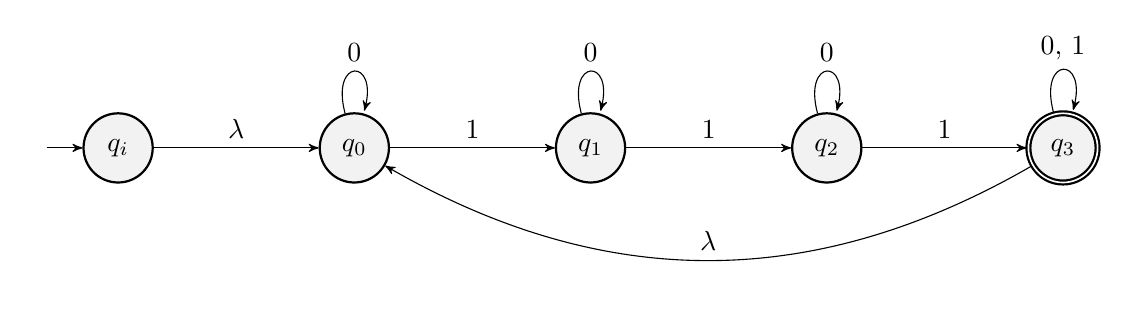
\begin{tikzpicture}[node distance=3cm]
    % Original DFA
    \node[state] (q0) {$q_0$};
    \node[state, right of=q0] (q1) {$q_1$};
    \node[state, right of=q1] (q2) {$q_2$};
    \node[state, accepting, right of=q2] (q3) {$q_3$};
    \draw 
    (q0) edge[loop above] node{0} (q0)
    (q0) edge[above] node{1} (q1)
    (q1) edge[loop above] node{0} (q1)
    (q1) edge[above] node{1} (q2)
    (q2) edge[loop above] node{0} (q2)
    (q2) edge[above] node{1} (q3)
    (q3) edge[loop above] node{0, 1} (q3);

    % Star construction
    \node[state, initial, xshift = -3cm] (qi) {$q_i$};
    \draw 
    (q3) edge[bend left, above] node{$\lambda$} (q0)
    (qi) edge[above] node{$\lambda$} (q0);
  \end{tikzpicture}
  \caption{$DFA_{L}$}
\end{figure}


\section*{1.12}
$D = \{ w| w \text{ contains an even number of } a \text{'s and an odd number of } b \text{'s and does not contain the substring } ab \}$. Give a DFA with five states that recognizes $D$ and a regular expression that generates $D$. (Suggestion: Describe $D$ more simply.)


\begin{center}
  \underline{Solution:}
\end{center}

Since the substring $ab$ is not allowed, then all $b$ symbols (at least one $b$ symbol must exist) must come at the front before all $a$ symbols (if any).
\newline

\underline{Regular Expression:}
\begin{align*}
  L = (bb)^*b(aa)^*
\end{align*}

\underline{Automaton (DFA):}

\begin{figure}[H]
  \centering
  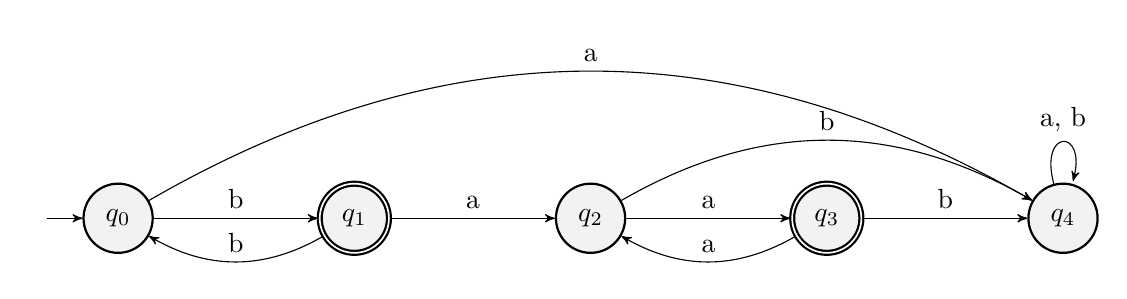
\begin{tikzpicture}[node distance=3cm]
    % Original DFA
    \node[state, initial] (q0) {$q_0$};
    \node[state, accepting, right of=q0] (q1) {$q_1$};
    \node[state, right of=q1] (q2) {$q_2$};
    \node[state, accepting, right of=q2] (q3) {$q_3$};
    \node[state, right of=q3] (q4) {$q_4$};
    \draw 
    (q0) edge[bend left, above] node{a} (q4)
    (q0) edge[above] node{b} (q1)
    (q1) edge[above] node{a} (q2)
    (q1) edge[bend left, above] node{b} (q0)
    (q2) edge[above] node{a} (q3)
    (q2) edge[bend left, above] node{b} (q4)
    (q3) edge[bend left, above] node{a} (q2)
    (q3) edge[above] node{b} (q4)
    (q4) edge[loop above] node{a, b} (q4);
  \end{tikzpicture}
  \caption{$DFA_{L}$}
\end{figure}


\section*{1.13}
Let $F$ be the language of all strings over $\{0,1\}$ that do not contain a pair of $1$s that are separated by an odd number of symbols.
Give the state diagram of a DFA with five states that recognizes $F$.
(You may find it helpful first to find a 4-state NFA for the complement of $F$.)

\begin{center}
  \underline{Solution:}
\end{center}

\begin{figure}[H]
  \centering
  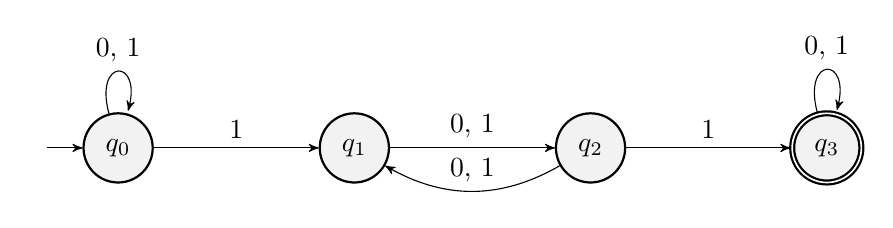
\begin{tikzpicture}
    \node[state, initial] (q0) {$q_0$};
    \node[state, right of=q0] (q1) {$q_1$};
    \node[state, right of=q1] (q2) {$q_2$};
    \node[state, accepting, right of=q2] (q3) {$q_3$};
    \draw 
    (q0) edge[loop above] node{0, 1} (q0)
    (q0) edge[above] node{1} (q1)
    (q1) edge[above] node{0, 1} (q2)
    (q2) edge[bend left, above] node{0, 1} (q1)
    (q2) edge[above] node{1} (q3)
    (q3) edge[loop above] node{0, 1} (q3);
  \end{tikzpicture}
  \caption{$NFA_{F^c}$}
\end{figure}

\begin{figure}[H]
  \centering
  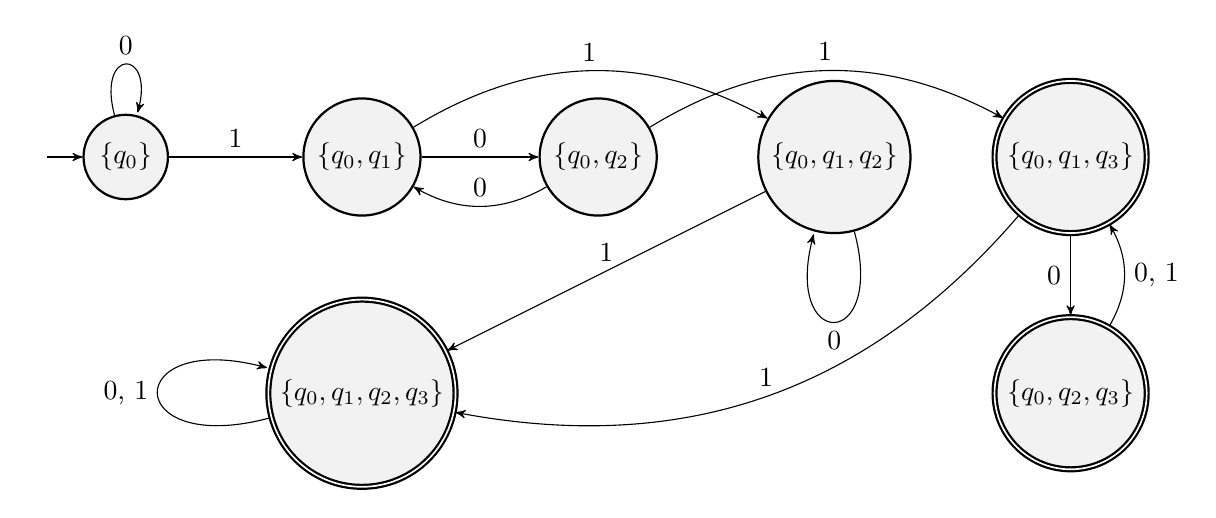
\begin{tikzpicture}
    \node[state, initial] (q0) {$\{q_0\}$};
    \node[state, right of=q0] (q1) {$\{q_0, q_1\}$};
    \node[state, right of=q1] (q2) {$\{q_0, q_2\}$};
    \node[state, right of=q2] (q3) {$\{q_0, q_1, q_2\}$};
    \node[state, accepting, right of=q3] (q4) {$\{q_0, q_1, q_3\}$};
    \node[state, accepting, below of=q1] (q5) {$\{q_0, q_1, q_2, q_3\}$};
    \node[state, accepting, below of=q4] (q6) {$\{q_0, q_2, q_3\}$};
    \draw 
    (q0) edge[loop above] node{0} (q0)
    (q0) edge[above] node{1} (q1)
    (q1) edge[above] node{0} (q2)
    (q1) edge[bend left, above] node{1} (q3)
    (q2) edge[bend left, above] node{0} (q1)
    (q2) edge[bend left, above] node{1} (q4)
    (q3) edge[loop below] node{0} (q3)
    (q3) edge[above] node{1} (q5)
    (q4) edge[left] node{0} (q6)
    (q4) edge[bend left, above] node{1} (q5)
    (q5) edge[loop left] node{0, 1} (q5)
    (q6) edge[bend right, right] node{0, 1} (q4);
  \end{tikzpicture}
  \caption{$DFA_{F^c}$}
\end{figure}

All three accepting states can be merged into one accepting state (since transitions from any accepting state lead to another accepting state).

\begin{figure}[H]
  \centering
  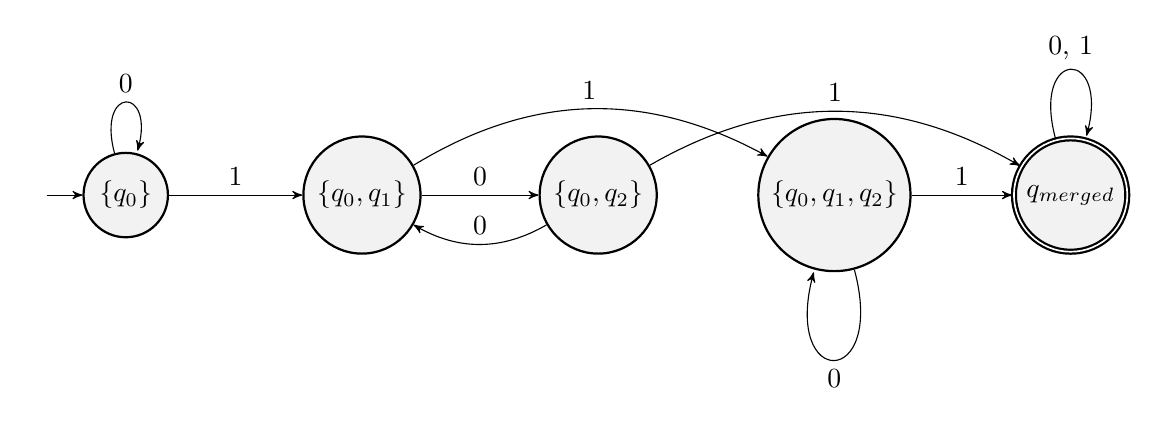
\begin{tikzpicture}
    \node[state, initial] (q0) {$\{q_0\}$};
    \node[state, right of=q0] (q1) {$\{q_0, q_1\}$};
    \node[state, right of=q1] (q2) {$\{q_0, q_2\}$};
    \node[state, right of=q2] (q3) {$\{q_0, q_1, q_2\}$};
    \node[state, accepting, right of=q3] (qm) {$q_{merged}$};
    \draw 
    (q0) edge[loop above] node{0} (q0)
    (q0) edge[above] node{1} (q1)
    (q1) edge[above] node{0} (q2)
    (q1) edge[bend left, above] node{1} (q3)
    (q2) edge[bend left, above] node{0} (q1)
    (q2) edge[bend left, above] node{1} (qm)
    (q3) edge[loop below] node{0} (q3)
    (q3) edge[above] node{1} (qm)
    (qm) edge[loop above] node{0, 1} (qm);
  \end{tikzpicture}
  \caption{$DFA_{F^c}$ (Merged Accepting States)}
\end{figure}

\begin{figure}[H]
  \centering
  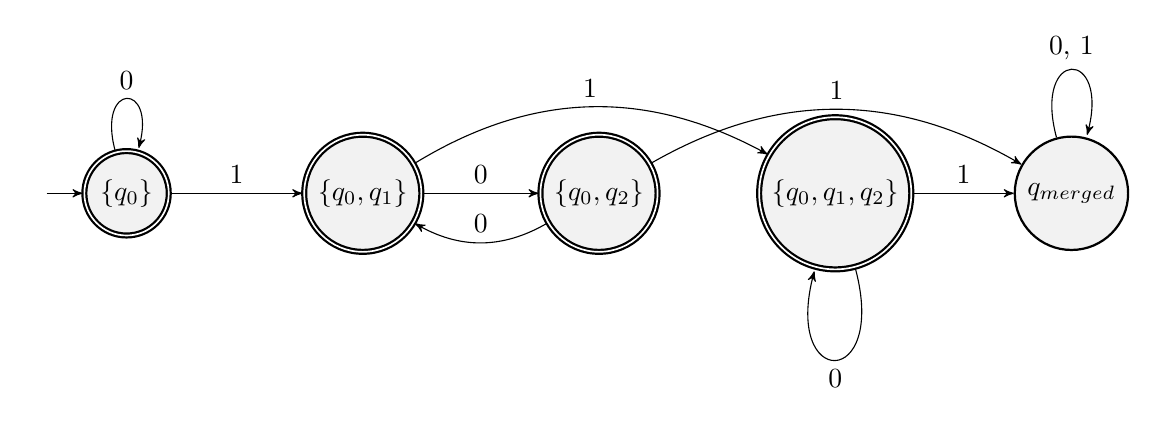
\begin{tikzpicture}
    \node[state, initial, accepting] (q0) {$\{q_0\}$};
    \node[state, accepting, right of=q0] (q1) {$\{q_0, q_1\}$};
    \node[state, accepting, right of=q1] (q2) {$\{q_0, q_2\}$};
    \node[state, accepting, right of=q2] (q3) {$\{q_0, q_1, q_2\}$};
    \node[state, right of=q3] (qm) {$q_{merged}$};
    \draw 
    (q0) edge[loop above] node{0} (q0)
    (q0) edge[above] node{1} (q1)
    (q1) edge[above] node{0} (q2)
    (q1) edge[bend left, above] node{1} (q3)
    (q2) edge[bend left, above] node{0} (q1)
    (q2) edge[bend left, above] node{1} (qm)
    (q3) edge[loop below] node{0} (q3)
    (q3) edge[above] node{1} (qm)
    (qm) edge[loop above] node{0, 1} (qm);
  \end{tikzpicture}
  \caption{$DFA_{F}$}
\end{figure}


\section*{1.16}
Use the construction given in Theorem 1.39 to convert the following two nondeterministic
finite automata to equivalent deterministic finite automata.

\subsection*{b.}
\begin{center}
  \underline{Solution:}
\end{center}

\begin{figure}[H]
  \centering
  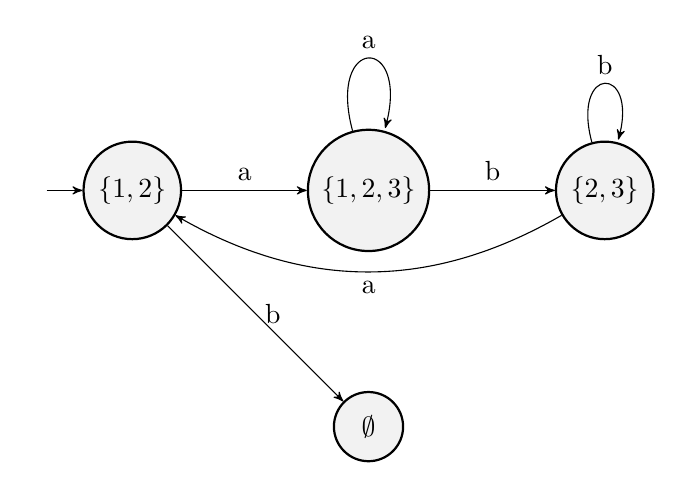
\begin{tikzpicture}
    \node[state, initial] (q0) {$\{1, 2\}$};
    \node[state, right of=q0] (q1) {$\{1, 2, 3\}$};
    \node[state, below of=q1] (q2) {$\emptyset$};
    \node[state, right of=q1] (q3) {$\{2, 3\}$};
    \draw 
    (q0) edge[above] node{a} (q1)
    (q0) edge[right] node{b} (q2)
    (q1) edge[loop above] node{a} (q1)
    (q1) edge[above] node{b} (q3)
    (q3) edge[bend left, below] node{a} (q0)
    (q3) edge[loop above] node{b} (q3);
  \end{tikzpicture}
  \caption{$DFA$}
\end{figure}


\section*{1.21}
Use the procedure described in Lemma 1.60 to convert the following finite automata to regular expressions.

\subsection*{b.}

\begin{figure}[H]
  \centering
  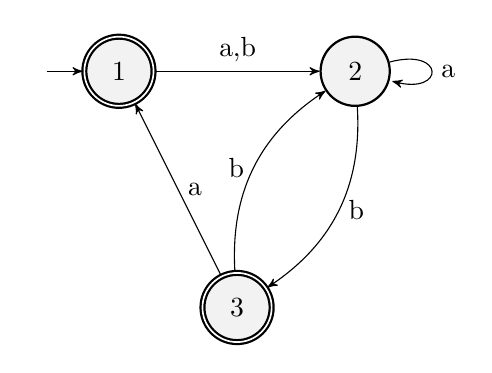
\begin{tikzpicture}
    \node[state, initial, accepting] (q1) {$1$};
    \node[state, right of=q1] (q2) {$2$};
    \node[state, accepting, below of=q1, xshift=1.5cm] (q3) {$3$};
    \draw 
    (q1) edge[above] node{a,b} (q2)
    (q2) edge[loop right] node{a} (q2)
    (q2) edge[bend left, right] node{b} (q3)
    (q3) edge[right] node{a} (q1)
    (q3) edge[bend left, left] node{b} (q2);
  \end{tikzpicture}
  \caption{$DFA$}
\end{figure}

\begin{center}
  \underline{Solution:}
\end{center}

To find the equivalent regular expression, we transform the DFA into the equivalent GDFA.
\newline

\noindent
We start by introducing a new initial state and a new accepting state:

\begin{figure}[H]
  \centering
  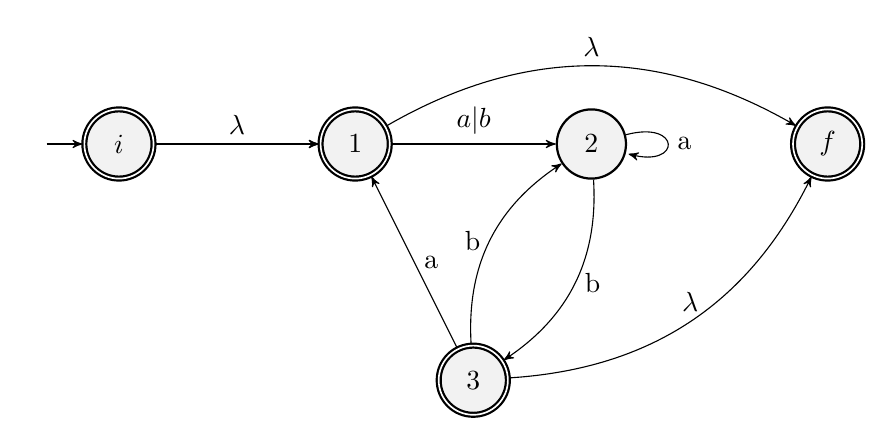
\begin{tikzpicture}
    \node[state, initial, accepting] (qi) {$i$};
    \node[state, initial, accepting, right of=qi] (q1) {$1$};
    \node[state, right of=q1] (q2) {$2$};
    \node[state, accepting, below of=q1, xshift=1.5cm] (q3) {$3$};
    \node[state, accepting, right of=q2] (qf) {$f$};

    \draw 
    (q1) edge[above] node{$a|b$} (q2)
    (q2) edge[loop right] node{a} (q2)
    (q2) edge[bend left, right] node{b} (q3)
    (q3) edge[right] node{a} (q1)
    (q3) edge[bend left, left] node{b} (q2);

    \draw
    (qi) edge[above] node{$\lambda$} (q1)
    (q1) edge[bend left, above] node{$\lambda$} (qf)
    (q3) edge[bend right, above] node{$\lambda$} (qf);
  \end{tikzpicture}
  \caption{$GDFA_1$}
\end{figure}

Next, we eliminate state $2$:
\begin{figure}[H]
  \centering
  \begin{tikzpicture}
    \node[state, initial, accepting] (qi) {$i$};
    \node[state, initial, accepting, right of=qi] (q1) {$1$};
    \node[state, accepting, below of=q1, xshift=1.5cm] (q3) {$3$};
    \node[state, accepting, right of=q2] (qf) {$f$};

    \draw 
    (q3) edge[right] node{a} (q1);

    \draw
    (qi) edge[above] node{$\lambda$} (q1)
    (q1) edge[bend left, above] node{$\lambda$} (qf)
    (q3) edge[bend right, above] node{$\lambda$} (qf)
    (q1) edge[bend right, left] node{$\left[a^+|ba^*\right]\left(bb\right)^*a^*b$} (q3);
  \end{tikzpicture}
  \caption{$GDFA_2$}
\end{figure}

Next, we eliminate state $3$:
\begin{figure}[H]
  \centering
  \begin{tikzpicture}
    \node[state, initial, accepting] (qi) {$i$};
    \node[state, initial, accepting, right of=qi] (q1) {$1$};
    \node[state, accepting, right of=q2] (qf) {$f$};

    \draw
    (qi) edge[above] node{$\lambda$} (q1)
    (q1) edge[bend left, above] node{$\lambda$} (qf)
    (q1) edge[loop above] node{$\left[a^+|ba^*\right]\left(bb\right)^*a^*ba$} (q1)
    (q1) edge[bend right, below] node{$\left[a^+|ba^*\right]\left(bb\right)^*a^*b$} (qf);
  \end{tikzpicture}
  \caption{$GDFA_3$}
\end{figure}

Finally, we eliminate state $1$:
\begin{figure}[H]
  \centering
  \begin{tikzpicture}
    \node[state, initial, accepting] (qi) {$i$};
    \node[state, accepting, right of=q2] (qf) {$f$};

    \draw
    (qi) edge[above] node{$\biggl(\left[a^+|ba^*\right]\left(bb\right)^*a^*ba\biggr)^* \left[a^+|ba^*\right]\left(bb\right)^*a^*b$} (qf);
    
  \end{tikzpicture}
  \caption{$GDFA_4$}
\end{figure}

Therefore:
\begin{align*}
  R = \biggl(\left[a^+|ba^*\right]\left(bb\right)^*a^*ba\biggr)^* \left[a^+|ba^*\right]\left(bb\right)^*a^*b
\end{align*}


\section*{1.22}
In certain programming languages, comments appear between delimiters such as $/\#$ and $\#/$. Let C be the language of all valid delimited comment strings. A member of C must begin with $/\#$ and end with $\#/$ but have no intervening $\#/$. For simplicity, assume that the alphabet for C is $\Sigma = \{a, b, /, \#\}$.
\subsection*{a.}
Give a DFA that recognizes C.

\begin{center}
  \underline{Solution:}
\end{center}

\begin{figure}[H]
  \centering
  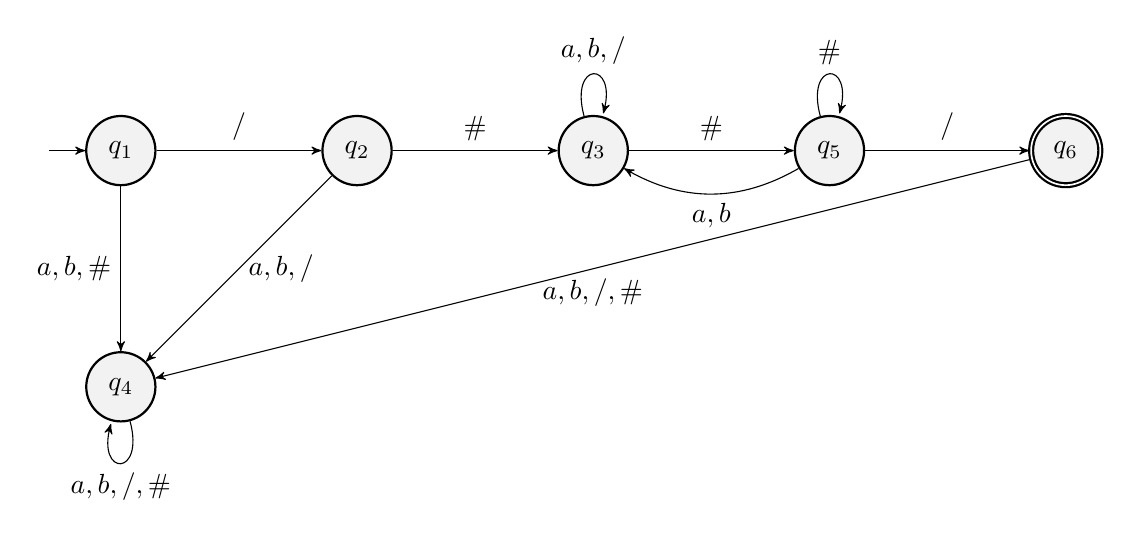
\begin{tikzpicture}
    \node[state, initial] (q1) {$q_1$};
    \node[state, right of=q1] (q2) {$q_2$};
    \node[state, right of=q2] (q3) {$q_3$};
    \node[state, below of=q1] (q4) {$q_4$};
    \node[state, right of=q3] (q5) {$q_5$};
    \node[state, accepting, right of=q5] (q6) {$q_6$};

    \draw
    (q1) edge[above] node{$/$} (q2)
    (q1) edge[left] node{$a, b, \#$} (q4)
    (q2) edge[above] node{$\#$} (q3)
    (q2) edge[right] node{$a, b, /$} (q4)
    (q3) edge[loop above] node{$a, b, /$} (q3)
    (q3) edge[above] node{$\#$} (q5)
    (q5) edge[bend left, below] node{$a, b$} (q3)
    (q5) edge[loop above] node{$\#$} (q3)
    (q5) edge[above] node{$/$} (q6)
    (q6) edge[below] node{$a, b, /, \#$} (q4)
    (q4) edge[loop below] node{$a, b, /, \#$} (q4);
  \end{tikzpicture}
  \caption{$DFA_C$}
\end{figure}


\subsection*{b.}
Give a regular expression that generates $C$.

\begin{center}
  \underline{Solution:}
\end{center}

To find the equivalent regular expression, we transform the DFA into the equivalent GDFA.

First, we eliminate $q_2$:
\begin{figure}[H]
  \centering
  \begin{tikzpicture}
    \node[state, initial] (q1) {$q_1$};
    \node[state, right of=q2] (q3) {$q_3$};
    \node[state, below of=q1] (q4) {$q_4$};
    \node[state, right of=q3] (q5) {$q_5$};
    \node[state, accepting, right of=q5] (q6) {$q_6$};

    \draw
    (q1) edge[above] node{$/ \#$} (q3)
    (q1) edge[left] node{$a, b, \#$} (q4)
    (q3) edge[loop above] node{$a, b, /$} (q3)
    (q3) edge[above] node{$\#$} (q5)
    (q5) edge[bend left, below] node{$a, b$} (q3)
    (q5) edge[loop above] node{$\#$} (q3)
    (q5) edge[above] node{$/$} (q6)
    (q6) edge[below] node{$a, b, /, \#$} (q4)
    (q4) edge[loop below] node{$a, b, /, \#$} (q4);
  \end{tikzpicture}
  \caption{$DFA_C$}
\end{figure}

Next, we eliminate $q_5$:
\begin{figure}[H]
  \centering
  \begin{tikzpicture}
    \node[state, initial] (q1) {$q_1$};
    \node[state, right of=q2] (q3) {$q_3$};
    \node[state, below of=q1] (q4) {$q_4$};
    \node[state, accepting, right of=q5] (q6) {$q_6$};

    \draw
    (q1) edge[above] node{$/ \#$} (q3)
    (q1) edge[left] node{$a, b, \#$} (q4)
    (q3) edge[loop above] node{$a, b, /$} (q3)
    (q3) edge[above] node{$ \biggl( \# | \#^+ \bigl( a | b\bigr) \# \biggr) /$} (q6)
    (q6) edge[below] node{$a, b, /, \#$} (q4)
    (q4) edge[loop below] node{$a, b, /, \#$} (q4);
  \end{tikzpicture}
  \caption{$DFA_C$}
\end{figure}

Next, we eliminate $q_3$:
\begin{figure}[H]
  \centering
  \begin{tikzpicture}
    \node[state, initial] (q1) {$q_1$};
    \node[state, below of=q1] (q4) {$q_4$};
    \node[state, accepting, right of=q5] (q6) {$q_6$};

    \draw
    (q1) edge[left] node{$a, b, \#$} (q4)
    (q1) edge[above] node{$ / \# \bigl( a, b, / \bigr)^* \biggl( \# | \#^+ \bigl( a | b\bigr) \# \biggr) /$} (q6)
    (q6) edge[below] node{$a, b, /, \#$} (q4)
    (q4) edge[loop below] node{$a, b, /, \#$} (q4);
  \end{tikzpicture}
  \caption{$DFA_C$}
\end{figure}

Finally, we eliminate $q_4$:
\begin{figure}[H]
  \centering
  \begin{tikzpicture}
    \node[state, initial] (q1) {$q_1$};
    \node[state, accepting, right of=q5] (q6) {$q_6$};

    \draw
    (q1) edge[above] node{$/ \# \bigl( a, b, / \bigr)^* \biggl( \# | \#^+ \bigl( a | b\bigr) \# \biggr) /$} (q6);
  \end{tikzpicture}
  \caption{$DFA_C$}
\end{figure}

\begin{align*}
  R = / \# \bigl( a, b, / \bigr)^* \biggl( \# | \#^+ \bigl( a | b\bigr) \# \biggr) /
\end{align*}


\section*{1.27}
Read the informal definition of the finite state transducer given in Exercise $1.24$. Give the state diagram of an FST with the following behavior. Its input and output alphabets are $\{0,1\}$. Its output string is identical to the input string on the even positions but inverted on the odd positions. For example, on input $0000111$ it should output $1010010$.

\begin{center}
  \underline{Solution:}
\end{center}

\begin{figure}[H]
  \centering
  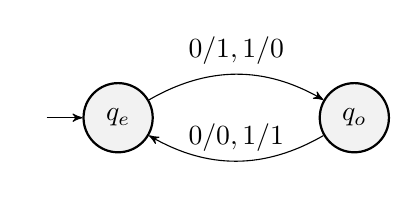
\begin{tikzpicture}
    \node[state, initial] (qe) {$q_e$};
    \node[state, right of=qe] (qo) {$q_o$};

    \draw
    (qe) edge[bend left, above] node{$0/1, 1/0$} (qo)
    (qo) edge[bend left, above] node{$0/0, 1/1$} (qe);
  \end{tikzpicture}
  \caption{$DFA$}
\end{figure}


\section*{1.28}
Convert the following regular expressions to NFAs using the procedure given in Theorem 1.54. In all parts, $\Sigma = \{a, b\}$.

\subsection*{a.}
\begin{align*}
  L=a\left(abb\right)^* \cup b
\end{align*}

\begin{center}
  \underline{Solution:}
\end{center}

\begin{figure}[H]
  \centering
  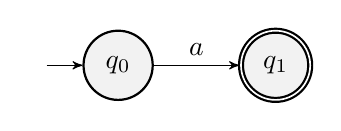
\begin{tikzpicture}[node distance=2cm, on grid, auto]
    \node[state, initial] (q0) {$q_0$};
    \node[state, accepting, right of=q0] (q1) {$q_1$};

    \draw
    (q0) edge[above] node{$a$} (q1);
  \end{tikzpicture}
  \caption{$NFA_{L=a}$}
\end{figure}

\begin{figure}[H]
  \centering
  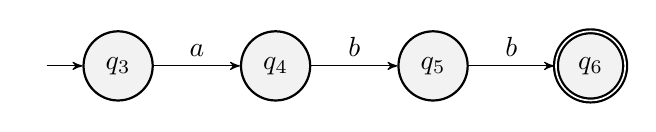
\begin{tikzpicture}[node distance=2cm, on grid, auto]
    \node[state, initial] (q3) {$q_3$};
    \node[state, right of=q3] (q4) {$q_4$};
    \node[state, right of=q4] (q5) {$q_5$};
    \node[state, accepting, right of=q5] (q6) {$q_6$};

    \draw
    (q3) edge[above] node{$a$} (q4)
    (q4) edge[above] node{$b$} (q5)
    (q5) edge[above] node{$b$} (q6);
  \end{tikzpicture}
  \caption{$NFA_{L=abb}$}
\end{figure}


\begin{figure}[H]
  \centering
  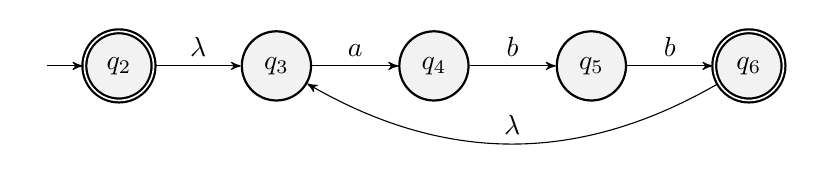
\begin{tikzpicture}[node distance=2cm, on grid, auto]
    \node[state, initial, accepting] (q2) {$q_2$};
    \node[state, right of=q2] (q3) {$q_3$};
    \node[state, right of=q3] (q4) {$q_4$};
    \node[state, right of=q4] (q5) {$q_5$};
    \node[state, accepting, right of=q5] (q6) {$q_6$};

    \draw
    (q3) edge[above] node{$a$} (q4)
    (q4) edge[above] node{$b$} (q5)
    (q5) edge[above] node{$b$} (q6);

    \draw
    (q2) edge[above] node{$\lambda$} (q3)
    (q6) edge[bend left, above] node{$\lambda$} (q3);
  \end{tikzpicture}
  \caption{$NFA_{L=\left(abb\right)^*}$}
\end{figure}

\begin{figure}[H]
  \centering
  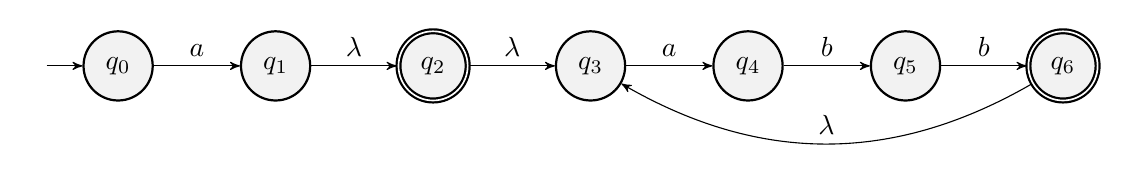
\begin{tikzpicture}[node distance=2cm, on grid, auto]
    \node[state, initial] (q0) {$q_0$};
    \node[state, right of=q0] (q1) {$q_1$};
    \node[state, accepting, right of=q1] (q2) {$q_2$};
    \node[state, right of=q2] (q3) {$q_3$};
    \node[state, right of=q3] (q4) {$q_4$};
    \node[state, right of=q4] (q5) {$q_5$};
    \node[state, accepting, right of=q5] (q6) {$q_6$};

    \draw
    (q0) edge[above] node{$a$} (q1);

    \draw
    (q3) edge[above] node{$a$} (q4)
    (q4) edge[above] node{$b$} (q5)
    (q5) edge[above] node{$b$} (q6);

    \draw
    (q2) edge[above] node{$\lambda$} (q3)
    (q6) edge[bend left, above] node{$\lambda$} (q3);

    \draw
    (q1) edge[above] node{$\lambda$} (q2);
  \end{tikzpicture}
  \caption{$NFA_{L=a\left(abb\right)^*}$}
\end{figure}

\begin{figure}[H]
  \centering
  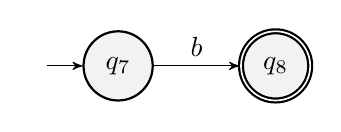
\begin{tikzpicture}[node distance=2cm, on grid, auto]
    \node[state, initial] (q7) {$q_7$};
    \node[state, accepting, right of=q7] (q8) {$q_8$};

    \draw
    (q7) edge[above] node{$b$} (q8);
  \end{tikzpicture}
  \caption{$NFA_{L=b}$}
\end{figure}

\begin{figure}[H]
  \centering
  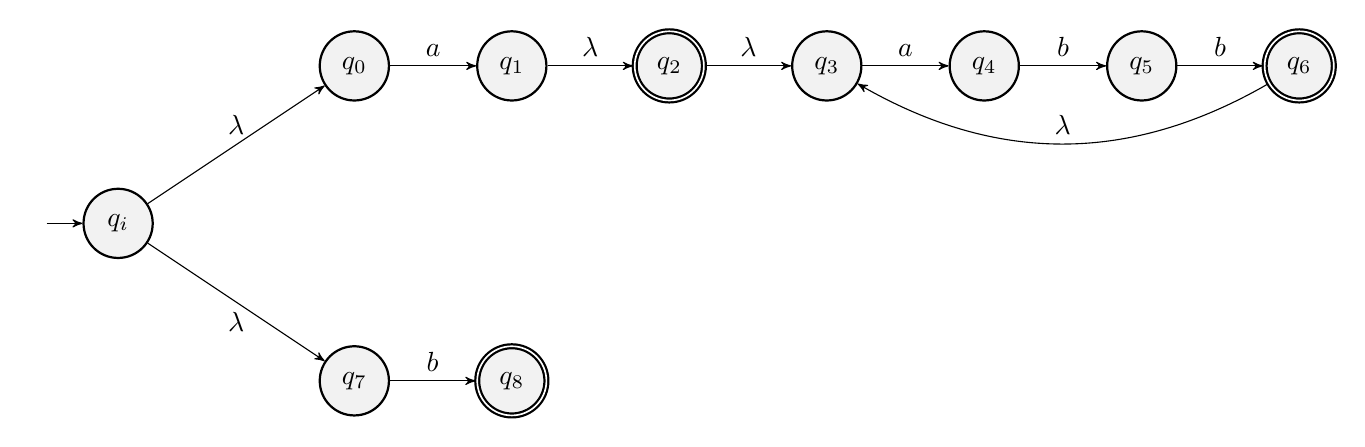
\begin{tikzpicture}[node distance=2cm, on grid, auto]
    \node[state, initial] (qi) {$q_i$};
    \node[state, right of=qi, yshift=2cm, xshift=1cm] (q0) {$q_0$};
    \node[state, right of=q0] (q1) {$q_1$};
    \node[state, accepting, right of=q1] (q2) {$q_2$};
    \node[state, right of=q2] (q3) {$q_3$};
    \node[state, right of=q3] (q4) {$q_4$};
    \node[state, right of=q4] (q5) {$q_5$};
    \node[state, accepting, right of=q5] (q6) {$q_6$};
    \node[state, right of=qi, yshift=-2cm, xshift=1cm] (q7) {$q_7$};
    \node[state, accepting, right of=q7] (q8) {$q_8$};

    \draw
    (q0) edge[above] node{$a$} (q1);

    \draw
    (q3) edge[above] node{$a$} (q4)
    (q4) edge[above] node{$b$} (q5)
    (q5) edge[above] node{$b$} (q6);

    \draw
    (q2) edge[above] node{$\lambda$} (q3)
    (q6) edge[bend left, above] node{$\lambda$} (q3);

    \draw
    (q1) edge[above] node{$\lambda$} (q2);

    \draw
    (q7) edge[above] node{$b$} (q8);

    \draw
    (qi) edge[above] node{$\lambda$} (q0)
    (qi) edge[below] node{$\lambda$} (q7);

  \end{tikzpicture}
  \caption{$NFA_{L=a\left(abb\right)^* \cup b}$}
\end{figure}


\section*{1.46}
Prove that the following languages are not regular. You may use the pumping lemma and the closure of the class of regular languages under union, intersection, and complement.

\subsection*{a.}
\begin{align*}
  L = \{ 0^n 1^m 0^n \: | \: m,n \geq 0 \}
\end{align*}

\begin{center}
  \underline{Solution:}
\end{center}

\begin{proof}
  $ $

  Suppose $L$ is regular. Then, there exists a pumping length $p$ for $L$.
  \newline

  Let $s = 0^p 1^p 0^p$.
  \newline

  Since $s \in L$ and $L$ is regular, then, by the pumping lemma:

  \indent
  i. $s = xyz$ 

  ii. $|y| > 0$

  iii. $|xy| \leq p$

  iv. $\forall i \geq 0$, the strings $xy^iz \in L$.
  \newline
  
  Conditions $ii, iii$ imply that $y$ consits of all zeros.
  \newline
  
  But this implies that the string $t = xy^2z$ contains more zeros on the left than on the right, and thus $t \notin L$.
  \newline

  This shows that $L$ cannot be pumped, and, thus, not regular.

\end{proof}


\section*{1.53}
Let $\Sigma = \{0, 1, +, =\}$ and

$ADD = \{x=y+z| x, y, z \text{ are binary integers, and } $x$ \text{ is the sum of } $y$ \text{ and } $z$\}$.

\begin{center}
  \underline{Solution:}
\end{center}

\begin{proof}
  $ $

  Suppose $ADD$ is regular. Then, there exists a pumping length $p$ for $ADD$.
  \newline

  Let $s$ be $1^p = 1^p + 0^p$.
  \newline

  Since $s \in ADD$ and $ADD$ is regular, then, by the pumping lemma:

  \indent
  i. $s = abc$ 

  ii. $|b| > 0$

  iii. $|ab| \leq p$

  iv. $\forall i \geq 0$, the strings $ab^ic \in ADD$.
  \newline
  
  Conditions $ii, iii$ imply that $b$ consits of all 1's.
  \newline
  
  But this implies that the string $t = xy^2z$ contains more 1's on the left than on the right (therefore, is not the valid result of an add operation), and thus $t \notin L$.
  \newline

  This shows that $L$ cannot be pumped, and, thus, not regular.

\end{proof}


\end{document}